\chapter{Διερεύνηση Χρονοσειράς Β}
\label{ch:step3}
\setcounter{page}{1}
\thispagestyle{fancy}

Για τη διερεύνηση της χρονοσειράς \textquote{Β} που αντιστοιχεί στο βίντεο \tl{No. 13} ακολουθήθηκαν παρόμοια βήματα με την χρονοσειρά \textquote{Β}. Έτσι, αρχικά δίνονται τα διαγράμματα ιστορίας, αυτοσυσχέτισης και μερικής αυτοσυσχέτισης της χρονοσειράς. Στη συνέχεια γίνεται σταθεροποίηση διασποράς και αφαίρεση της τάσης προκειμένου να γίνει στάσιμη η χρονοσειρά, παραθέτοντας και τα αντίστοιχα διαγράμματα της στάσιμης χρονοσειράς που προκύπτει.  

\section{Αρχική Ανάλυση}

Αρχικά, δίνεται το διάγραμμα ιστορίας της χρονοσειράς B, $\{Υ_b(t)\}$, ακολούθως.

\begin{figure}[H]
    \begin{center}
        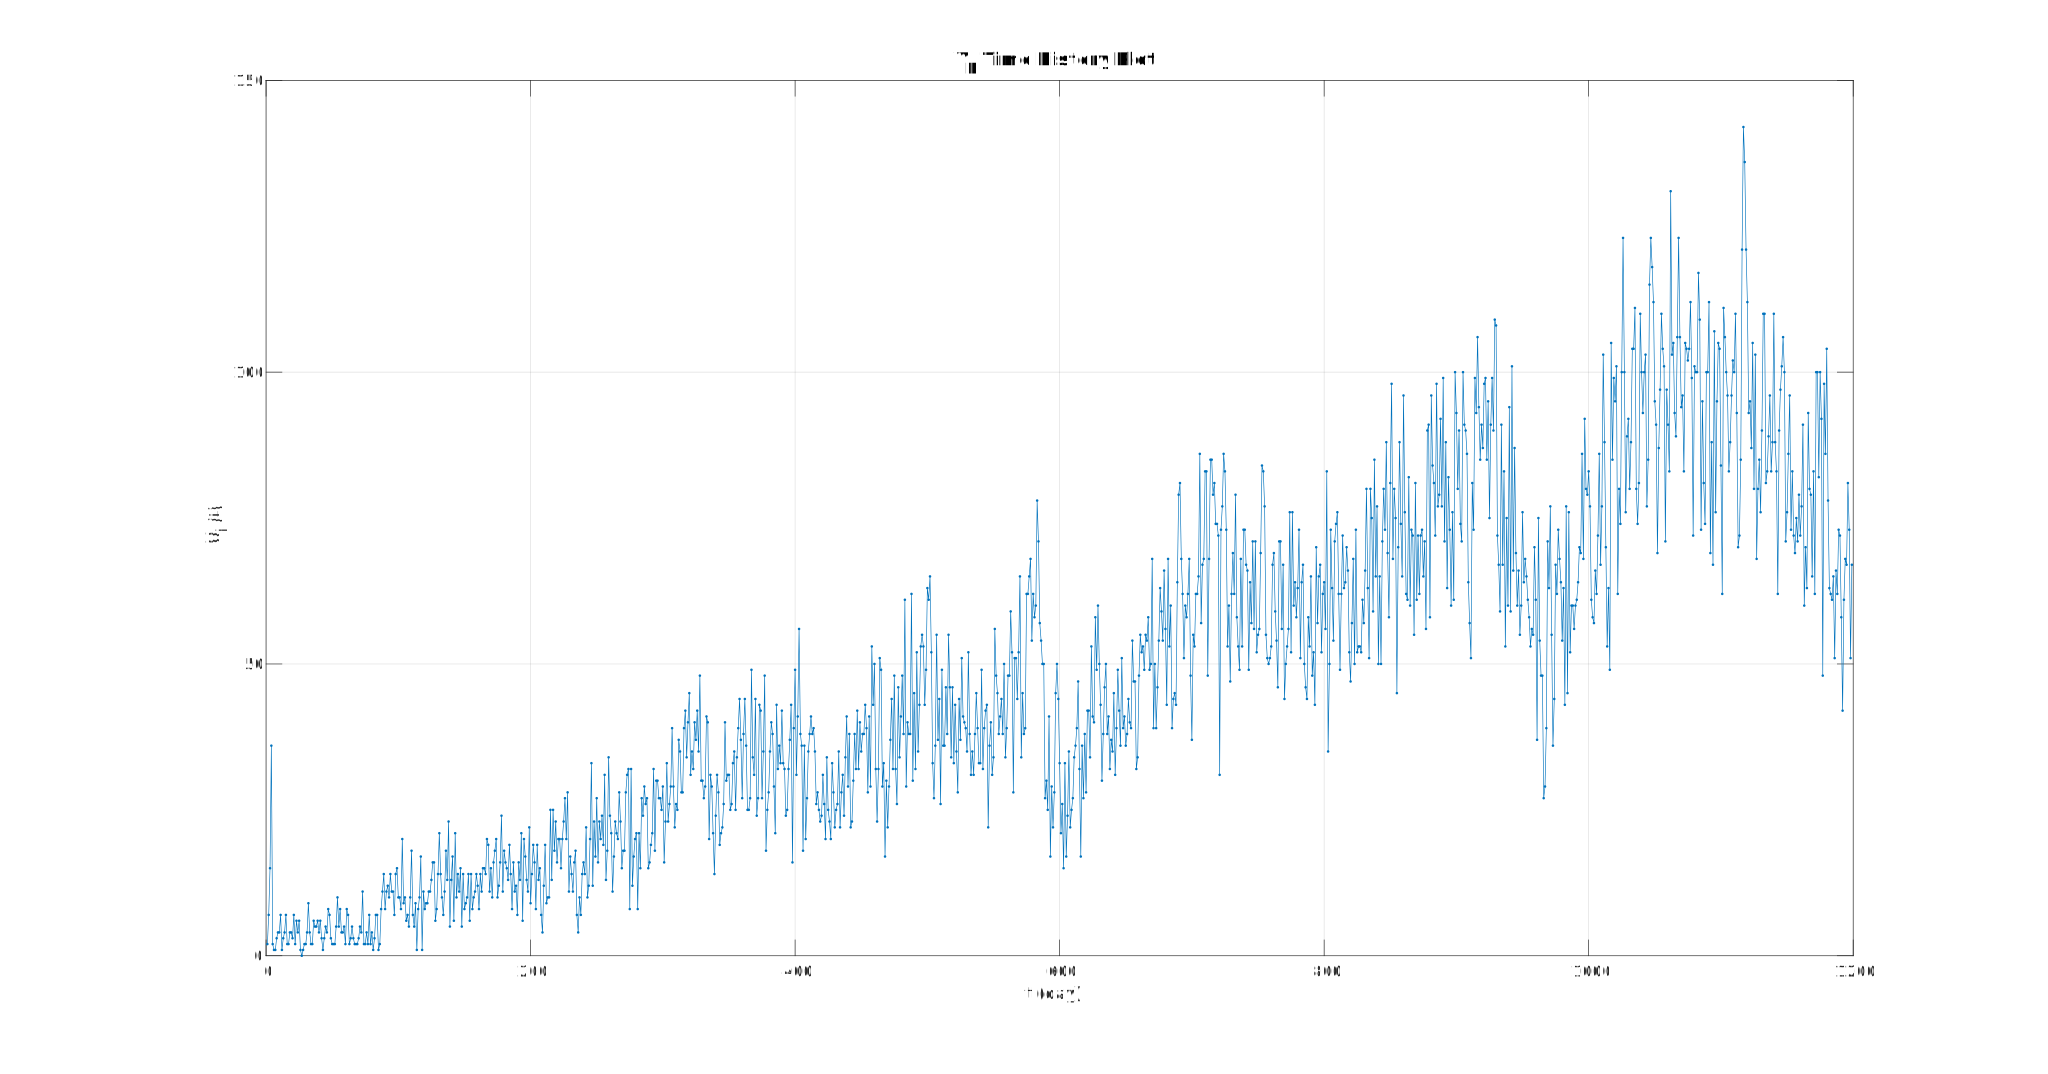
\includegraphics[width=\textwidth]{plots/yb_history.svg.pdf}
        \caption{Διάγραμμα ιστορίας της χρονοσειράς B, $\{Υ_b(t)\}$}
        \label{fig:yb_history}
    \end{center}
\end{figure}

Από το διάγραμμα ιστορίας της $\{Υ_b(t)\}$ φαίνεται πως η χρονοσειρά δεν είναι στάσιμη καθώς παρατηρείται έντονη αυξητική τάση. Αυτό επιβεβαιώνεται και από τα διαγράμματα της (δειγματικής) αυτοσυσχέτισης και (δειγματικής) μερικής αυτοσυσχέτισης που παρατίθενται ακολούθως:

\begin{figure}[H]
    \begin{center}
        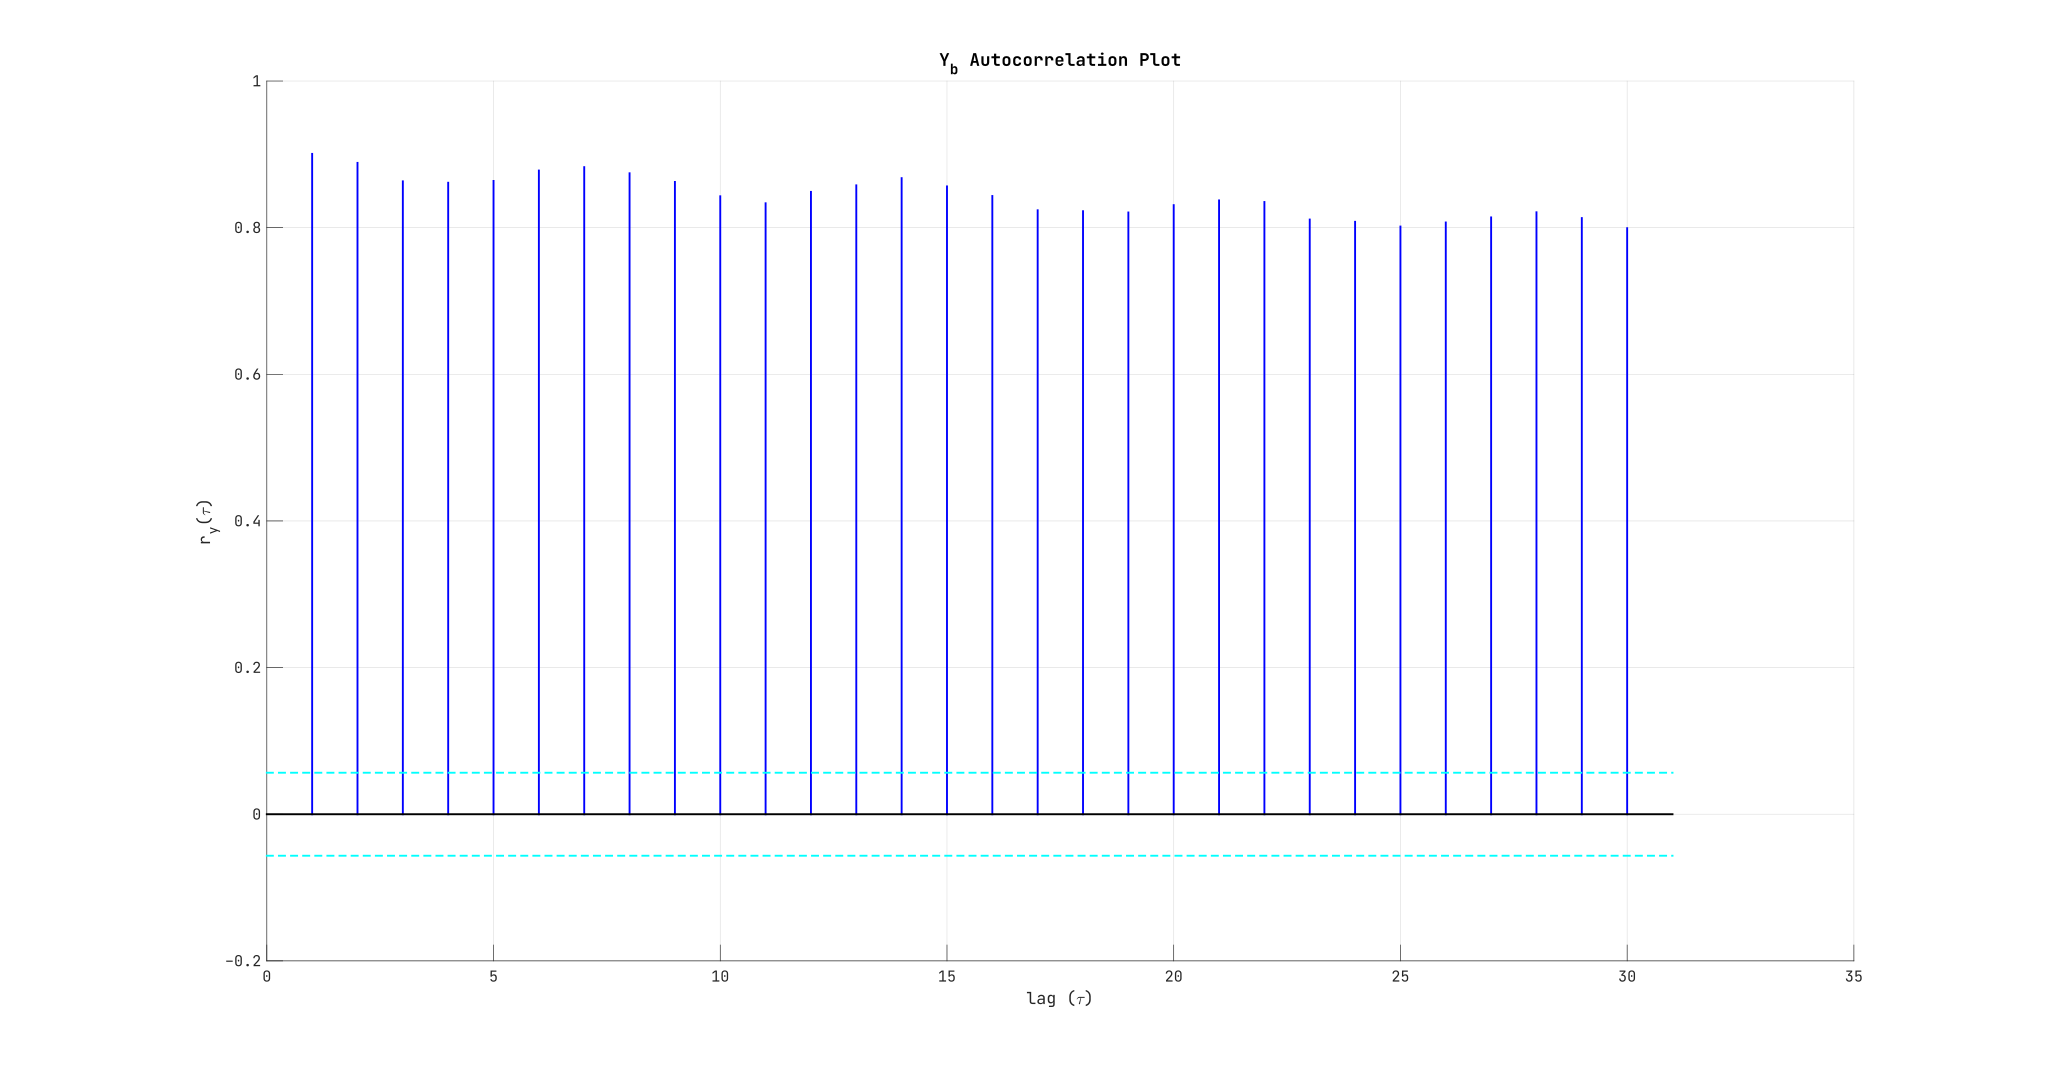
\includegraphics[width=\textwidth]{plots/yb_initial_autocorrelation.svg.pdf}
        \caption{Διάγραμμα (δειγματικής) αυτοσυσχέτισης της χρονοσειράς B, $r_y(\tau)$}
        \label{fig:yb_initial_autocorrelation}
    \end{center}
\end{figure}

\begin{figure}[H]
    \begin{center}
        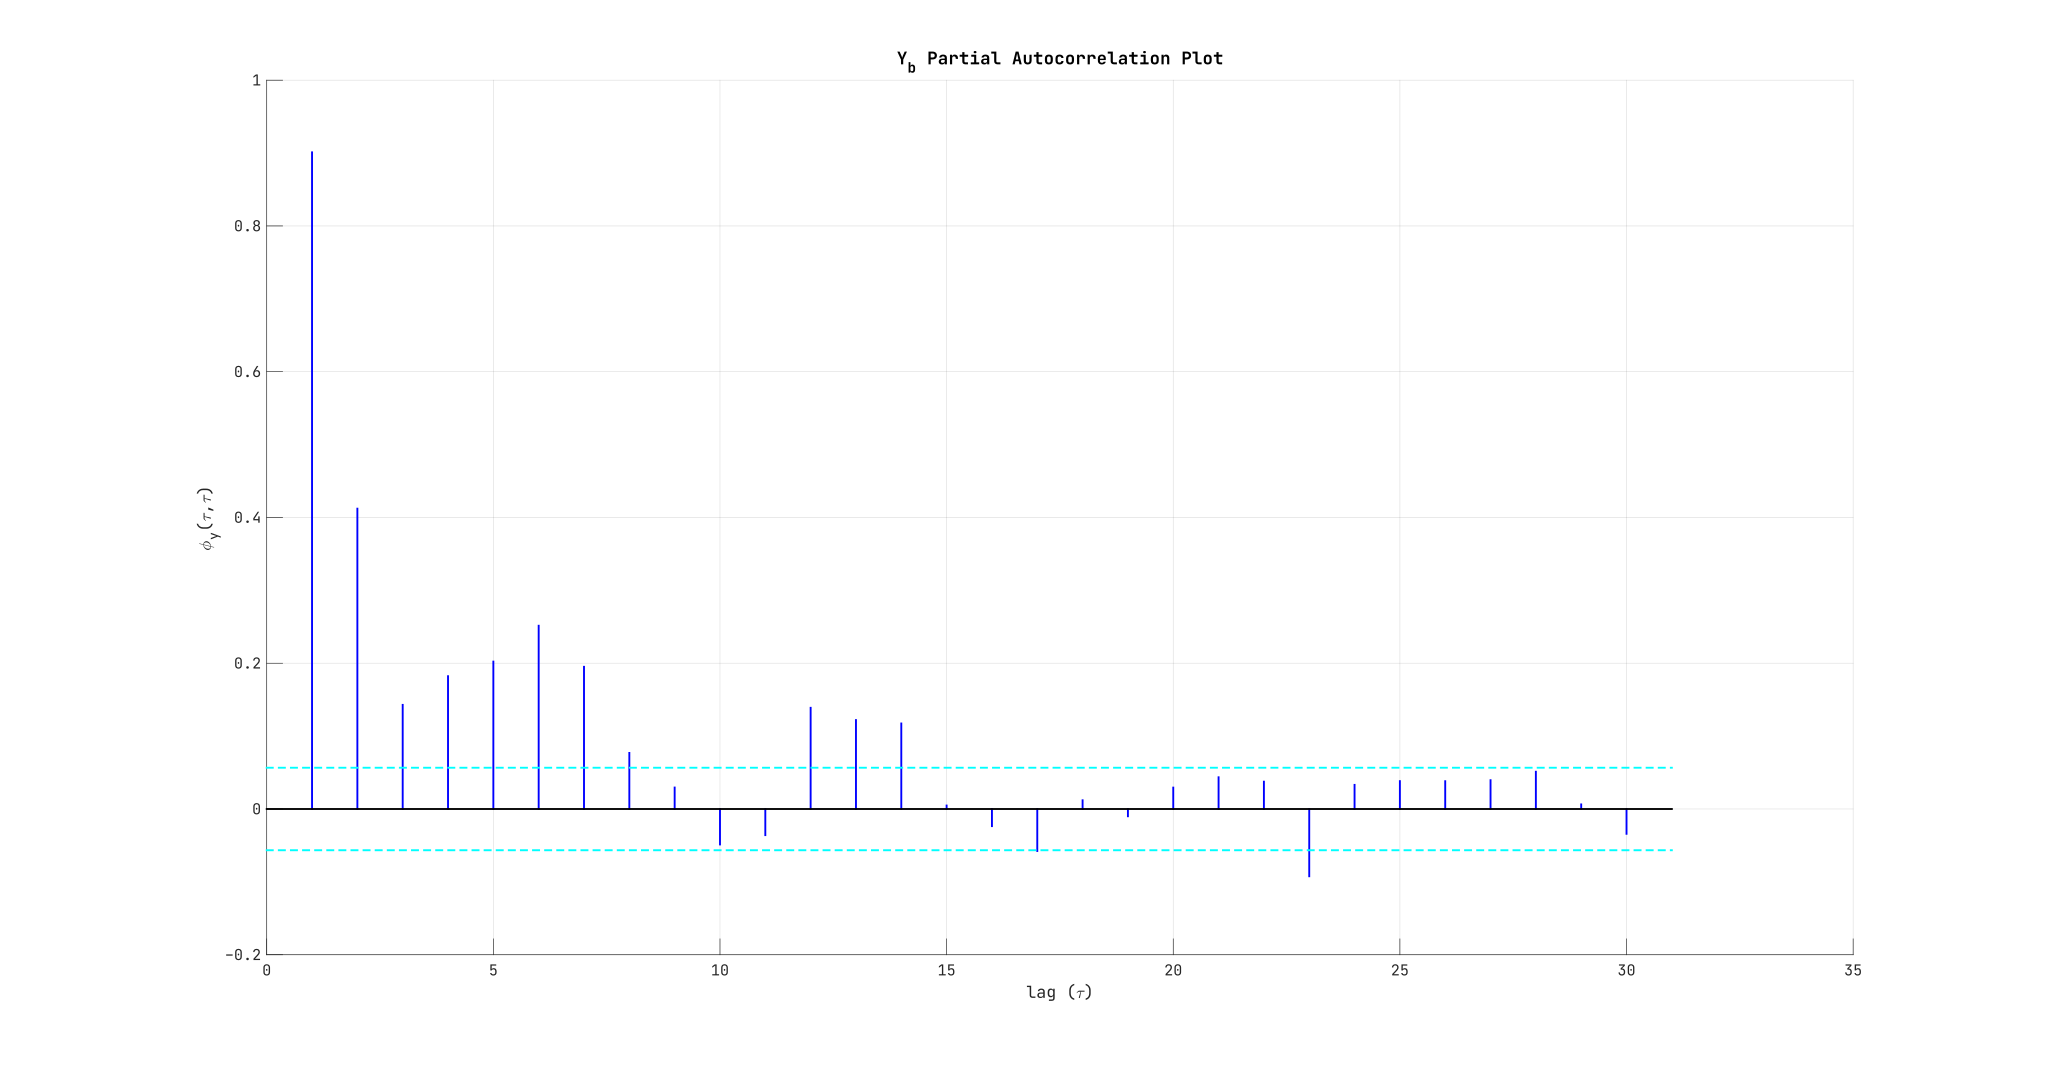
\includegraphics[width=\textwidth]{plots/yb_initial_partial_autocorrelation.svg.pdf}
        \caption{Διάγραμμα (δειγματικής) μερικής αυτοσυσχέτισης της χρονοσειράς B, $\phi_y(\tau)$}
        \label{fig:yb_initial_partial_autocorrelation}
    \end{center}
\end{figure}

Στα παραπάνω διαγράμματα έχουν σημειωθεί και τα όρια σημαντικότητας για επίπεδο εμπιστοσύνης 95\%. Ειδικά στο διάγραμμα αυτοσυσχέτισης φαίνεται έντονα η ύπαρξη τάσης καθώς η αυτοσυσχέτιση έχει υψηλές τιμές και φθίνει πολύ αργά. Η τάση, όπως φαίνεται από το διάγραμμα ιστορίας (σχήμα \ref{fig:yb_history}), είναι μάλλον στοχαστική και επομένως για να γίνει στάσιμη η χρονοσειρά θα πρέπει να εφαρμοστεί κάποια μέθοδος απαλοιφής της στοχαστικής τάσης (όπως η μέθοδος των πρώτων διαφορών).

\par Για λόγους πληρότητας, ωστόσο, παρουσιάζεται και η εκτίμηση της τάσης με φίλτρο κινούμενου μέσου όρου (\tl{MA}) τάξης 7, ώστε να κάνει \textquote{smoothing} με βάση τις εβδομαδιαίες προβολές του αντίστοιχου βίντεο.

\begin{figure}[H]
    \begin{center}
        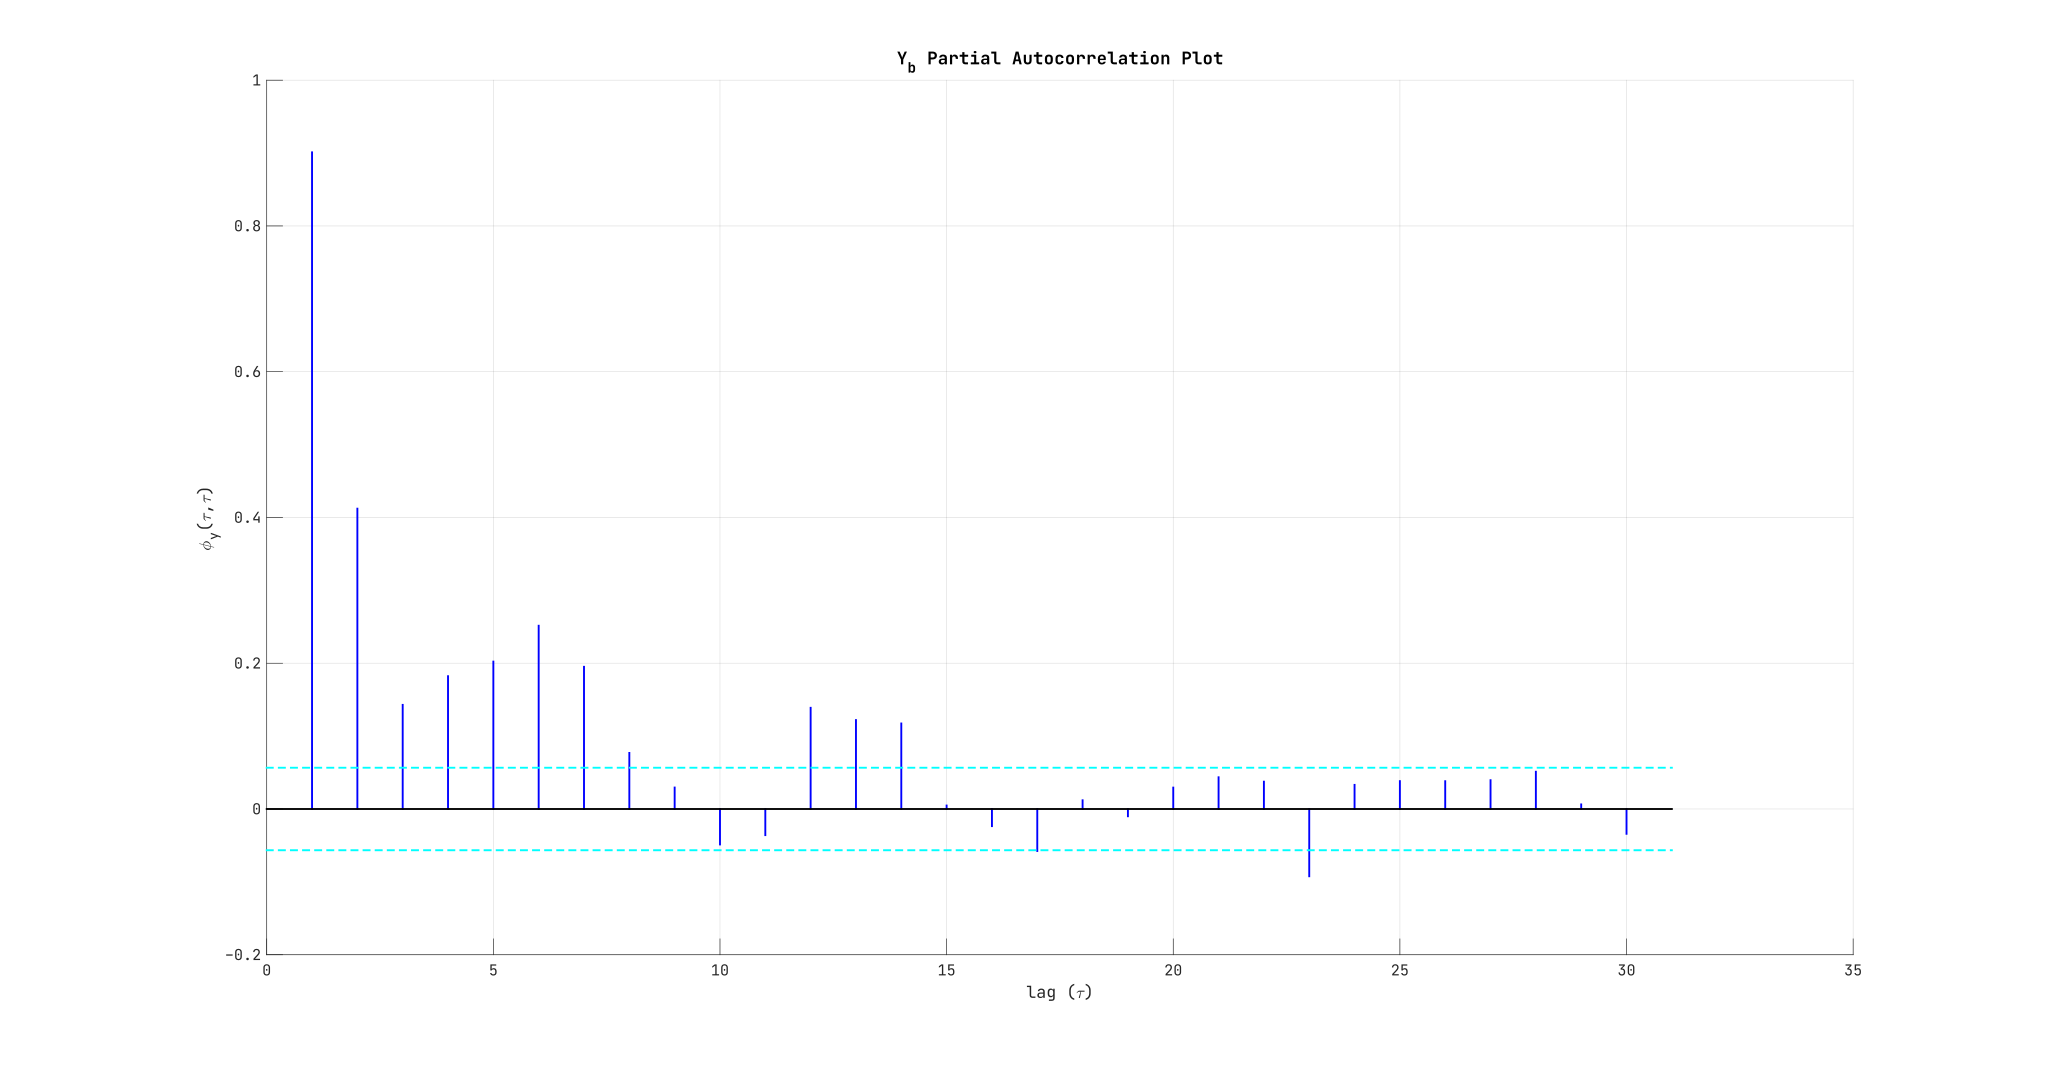
\includegraphics[width=\textwidth]{plots/yb_initial_partial_autocorrelation.svg.pdf}
        \caption{Διάγραμμα (δειγματικής) μερικής αυτοσυσχέτισης της χρονοσειράς B, $\phi_y(\tau)$}
        \label{fig:yb_initial_partial_autocorrelation}
    \end{center}
\end{figure}

\section{Απαλοιφή Στοχαστικής Τάσης}

Για την απαλοιφή της τάσης αρχικά δοκιμάστηκαν οι πρώτες διαφορές. Η χρονοσειρά που προκύπτει λοιπόν θα είναι:

\[ X_a(t) = Y_a(t) - Y_a(t-1) \]

Παρακάτω παρατίθεται το διάγραμμα ιστορίας της ${X_a(t)}$ όπου φαίνεται ότι ο μετασχηματισμός των πρώτων διαφορών έχει καταφέρει να απαλείψει τη στοαχαστική τάση και επομένως δεν υπάρχει η ανάγκη για επανάληψη της διαδικασίας (δηλαδή να πάρω διαφορές δεύτερης τάξης).

\begin{figure}[H]
    \begin{center}
        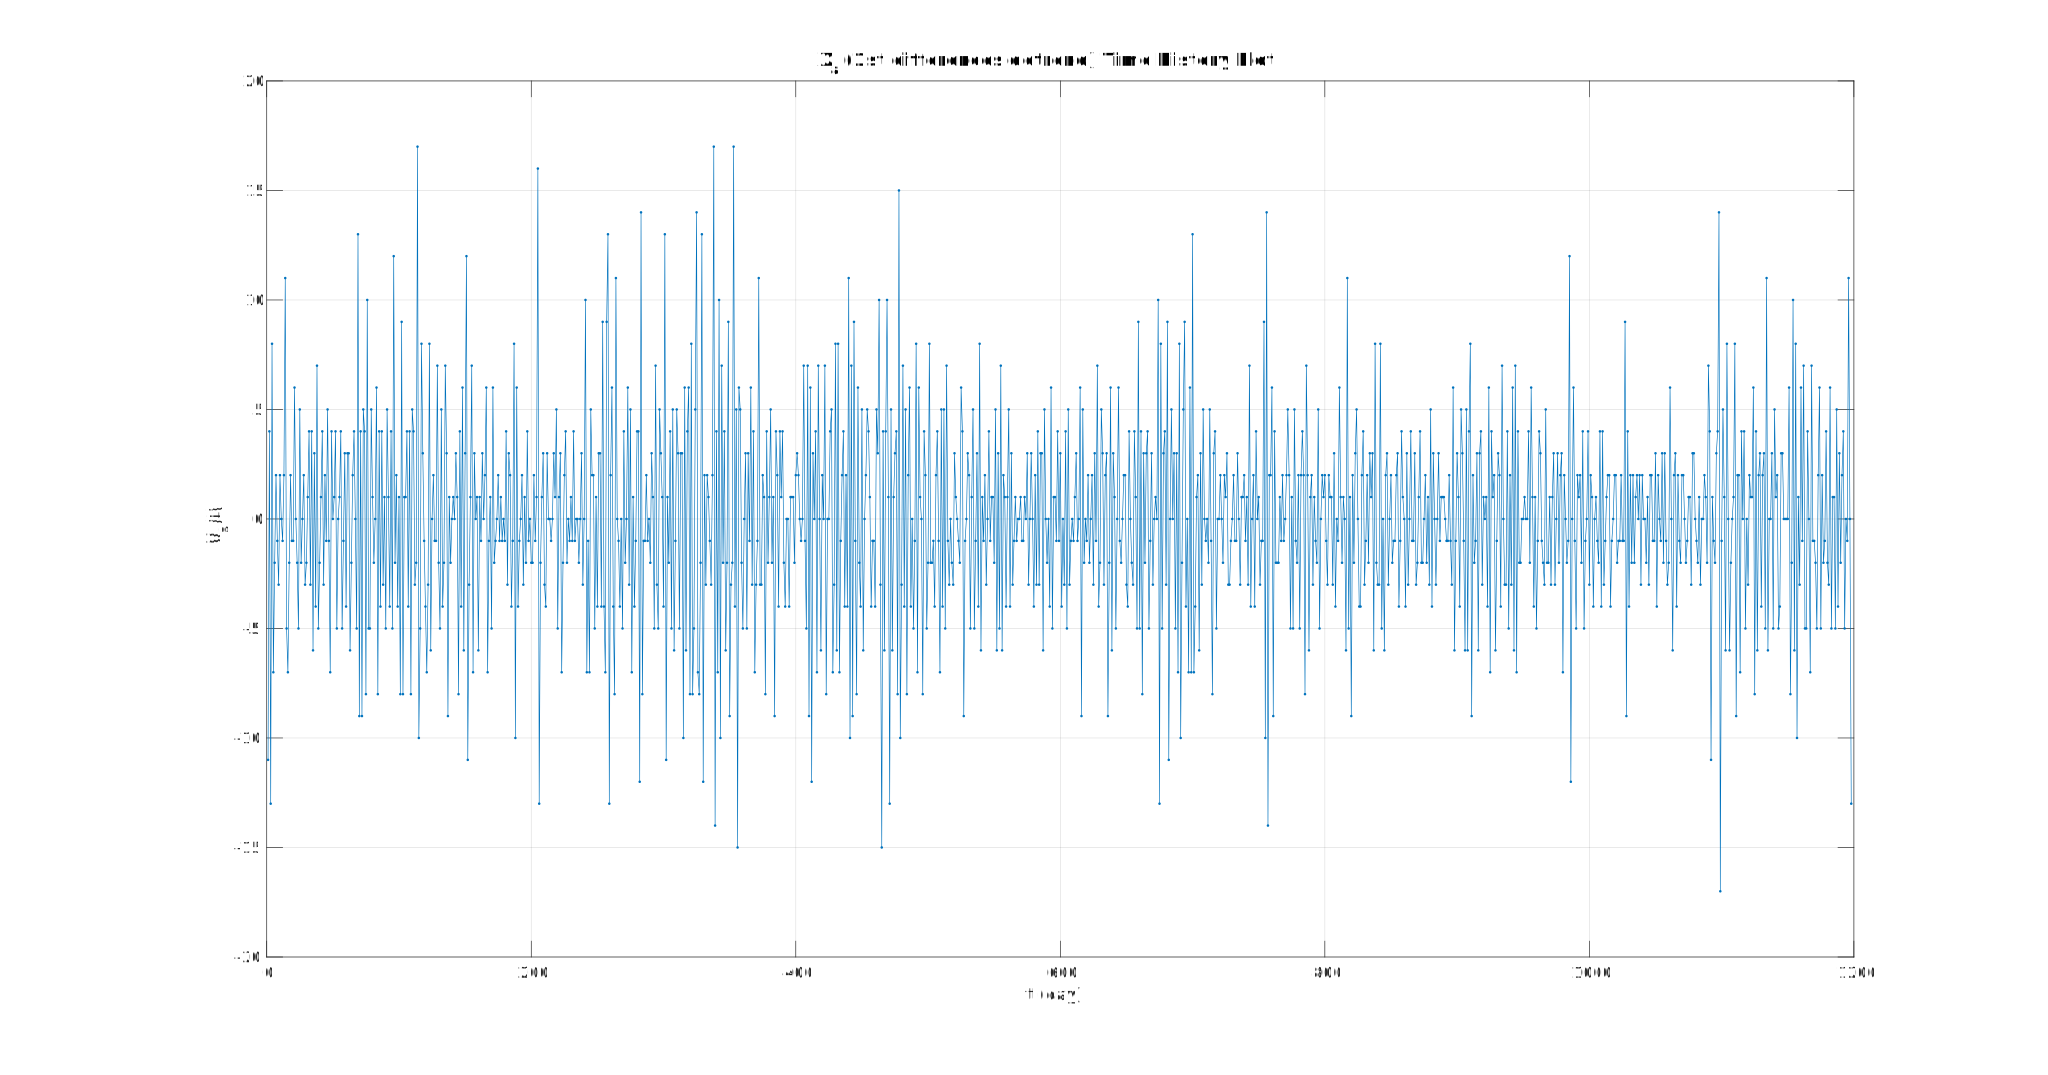
\includegraphics[width=\textwidth]{plots/xa_1st_differences_history.svg.pdf}
        \caption{Διάγραμμα ιστορίας στη χρονοσειρά των πρώτων διαφορών, $\{X_a(t)\}$}
        \label{fig:xa_1st_differences_history}
    \end{center}
\end{figure}

Ο παραπάνω ισχυρισμός περί απαλοιφής τάσης ενισχύεται και από τα ακόλουθα διαγράμματα δειγµατικής αυτοσυσχέτισης και δειγµατικής µερικής αυτοσυσχέτισης της χρονοσειράς των πρώτων διαφορών:

\begin{figure}[H]
    \begin{center}
        \includegraphics[width=\textwidth]{plots/xa_1st_differences_autocorrelation.svg.pdf}
        \caption{Διάγραμμα (δειγματικής) αυτοσυσχέτισης της χρονοσειράς πρώτων διαφορών, $r_x(\tau)$}
        \label{fig:xa_1st_differences_autocorrelation}
    \end{center}
\end{figure}

\begin{figure}[H]
    \begin{center}
        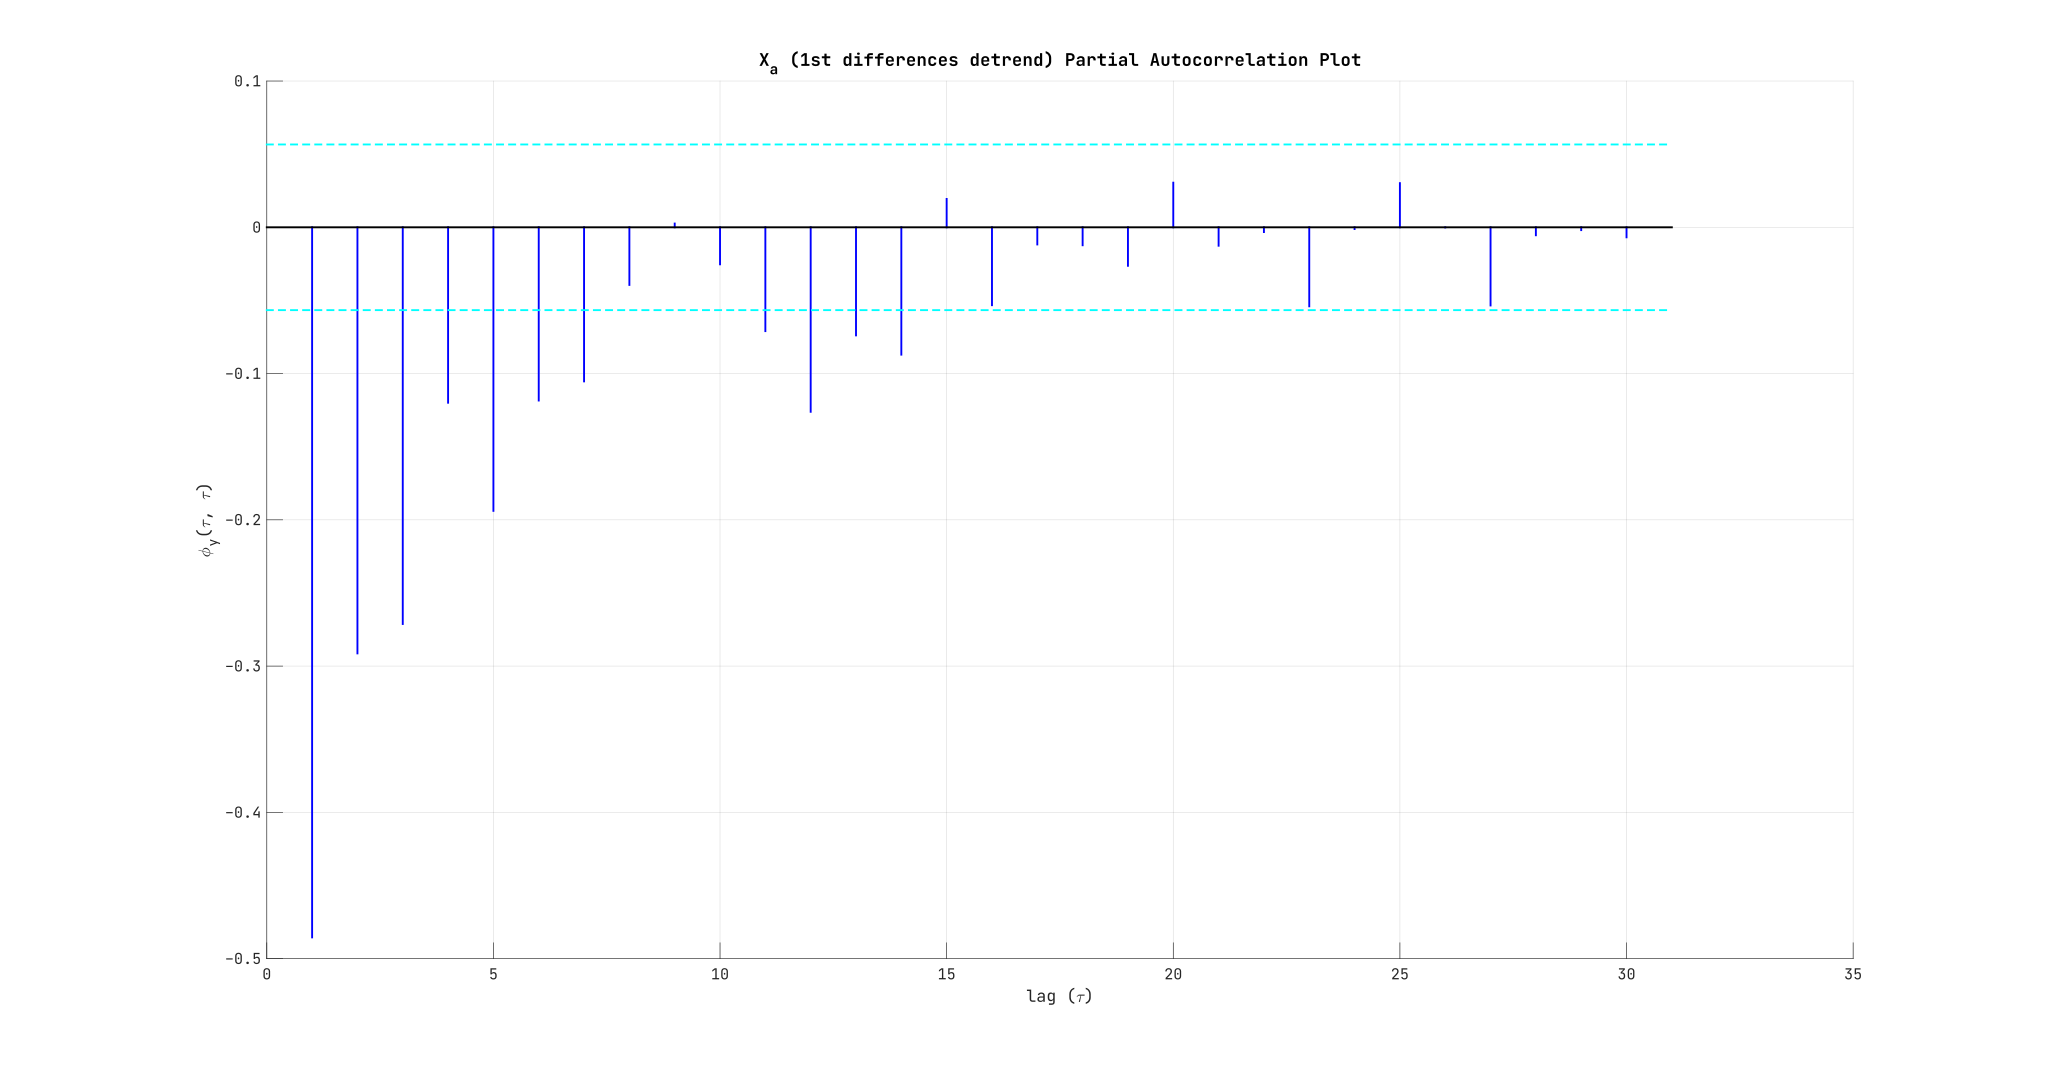
\includegraphics[width=\textwidth]{plots/xa_1st_differences_partial_autocorrelation.svg.pdf}
        \caption{Διάγραμμα (δειγματικής) μερικής αυτοσυσχέτισης της χρονοσειράς πρώτων διαφορών, $\phi_x(\tau)$}
        \label{fig:xa_1st_differences_partial_autocorrelation}
    \end{center}
\end{figure}

όπου αν και δεν φαίνεται η χρονοσειρά να παρουσιάζει αυτοσυσχέτιση λευκού θορύβου επίσης όμως δεν φαίνεται να παρουσιάζει και (στατιστικά) σημαντικές αυτοσυσχετίσεις (σχήμα \ref{fig:xa_1st_differences_autocorrelation}) ή αργή πτώση των τιμών. 

Σε ότι αφορά τη διασπορά της χρονοσειράς των πρώτων διαφορών, επιστρέφοντας στο διάγραμμα ιστορίας της (σχήμα \ref{fig:xa_1st_differences_history}) και συγκρίνοντάς το με το διάγραμμα ιστορίας της αρχικής χρονοσειράς (σχήμα \ref{fig:ya_history}) παρατηρούμε ότι η διασπορά της χρονοσειράς των πρώτων διαφορών φαίνεται να μεταβάλλεται κάπως σχετικά με τις \textquote{καμπλύλες} της τάσης της αρχικής χρονοσειράς. Επομένως, ίσως να ήταν σκόπιμο να προσπαθούσαμε να σταθεροποίσουμε τη διασπορά της προκύπτουσας χρονοσειράς ως προς τη τάση της αρχικής, κάτι που αναλύεται ακολούθως.

\section{Απαλοιφή Στοχαστικής Τάσης \& Σταθεροποίηση Διασποράς}

Η απαλοιφή της τάσης (\tl{detrending}) θεωρούμε πως έχει επιτευχθεί ικανοποιητικά παίρνοντας τις πρώτες διαφορές στην αρχική χρονοσειρά. Ωστόσο, πριν πάρουμε τις πρώτες διαφορές θα μας ενδιέφερε να απαλείψουμε την εξάρτηση της διασποράς της (αρχικής) χρονοσειράς από τη τάση. Για αυτό θα χρησιμοποιηθεί ο μετασχηματισμός των \tl{Box \& Cox} με $\lambda=0.5$ αφενός διότι φαίνεται η διασπορά να εξάρταται με ανάλογο (γραμμικό) τρόπο από τη τάση και αφετέρου επειδή η χρονοσειρά περιέχει μηδενικά δείγματα (καμία προβολή του αντίστοιχου βίντεο εκείνη την ημέρα) και άρα οι μετασχηματισμοί λογαρίθμου ή σχετικών μεταβολών δεν αποτελούν πρακτική λύση.

Ο μετασχηματισμός, λοιπόν, που χρησιμοποιηθήκε στην αρχική χρονοσειρά είναι αυτός της τετραγωνικής ρίζας. Δηλαδή, αρχικά η $\{Y_a(t)\}$ μετασχηματίστηκε σε:

\[ Y_a'(t) = \sqrt{Y_a(t)} \]

ενώ στη συνέχει χρησιμοποίηθηκαν οι πρώτες διαφορές για απαλοιφή της τάσης. Συνολικά, λοιπόν, ο μετασχηματισμός που υλοποιήθηκε για μετασχηματισμό της αρχικής χρονοσειράς σε στάσιμη είναι ο ακόλουθος:

\[ X_a(t) = \sqrt{Y_a(t)} - \sqrt{Y_a(t-1)} \]

με την $X_a(t)$ να είναι η στάσιμη εκδοχή της $Y_a(t)$. Παρακάτω, φαίνεται το διάγραμμα ιστορίας της (νέας) $X_a(t)$ όπου επιβεβαιώνεται η υπόθεσή μας για συσχέτιση της διασποράς με την τάση (αφού πλέον δεν φαίνεται αυτή η \textquote{κυματοειδής} μεταβολή της διασποράς). Θεωρούμε, δηλαδή, ότι εφαρμόζοντας το μετασχηματισμό της τετραγωνικής ρίζας στην αρχική χρονοσειρά \textbf{πριν} πάρουμε τις πρώτες διαφορές επιτυγχάνουμε την απεξάρτηση της διασποράς από την χρονικής μεταβολή της τάσης. Η χρονοσειρά ${X_a(t)}$ λοιπόν που προκύπτει αφενός δεν έχει εξάρτηση της διασποράς από την τάση και αφετέρου η στοχασστική τάση έχει απαλειφθεί.

\begin{figure}[H]
    \begin{center}
        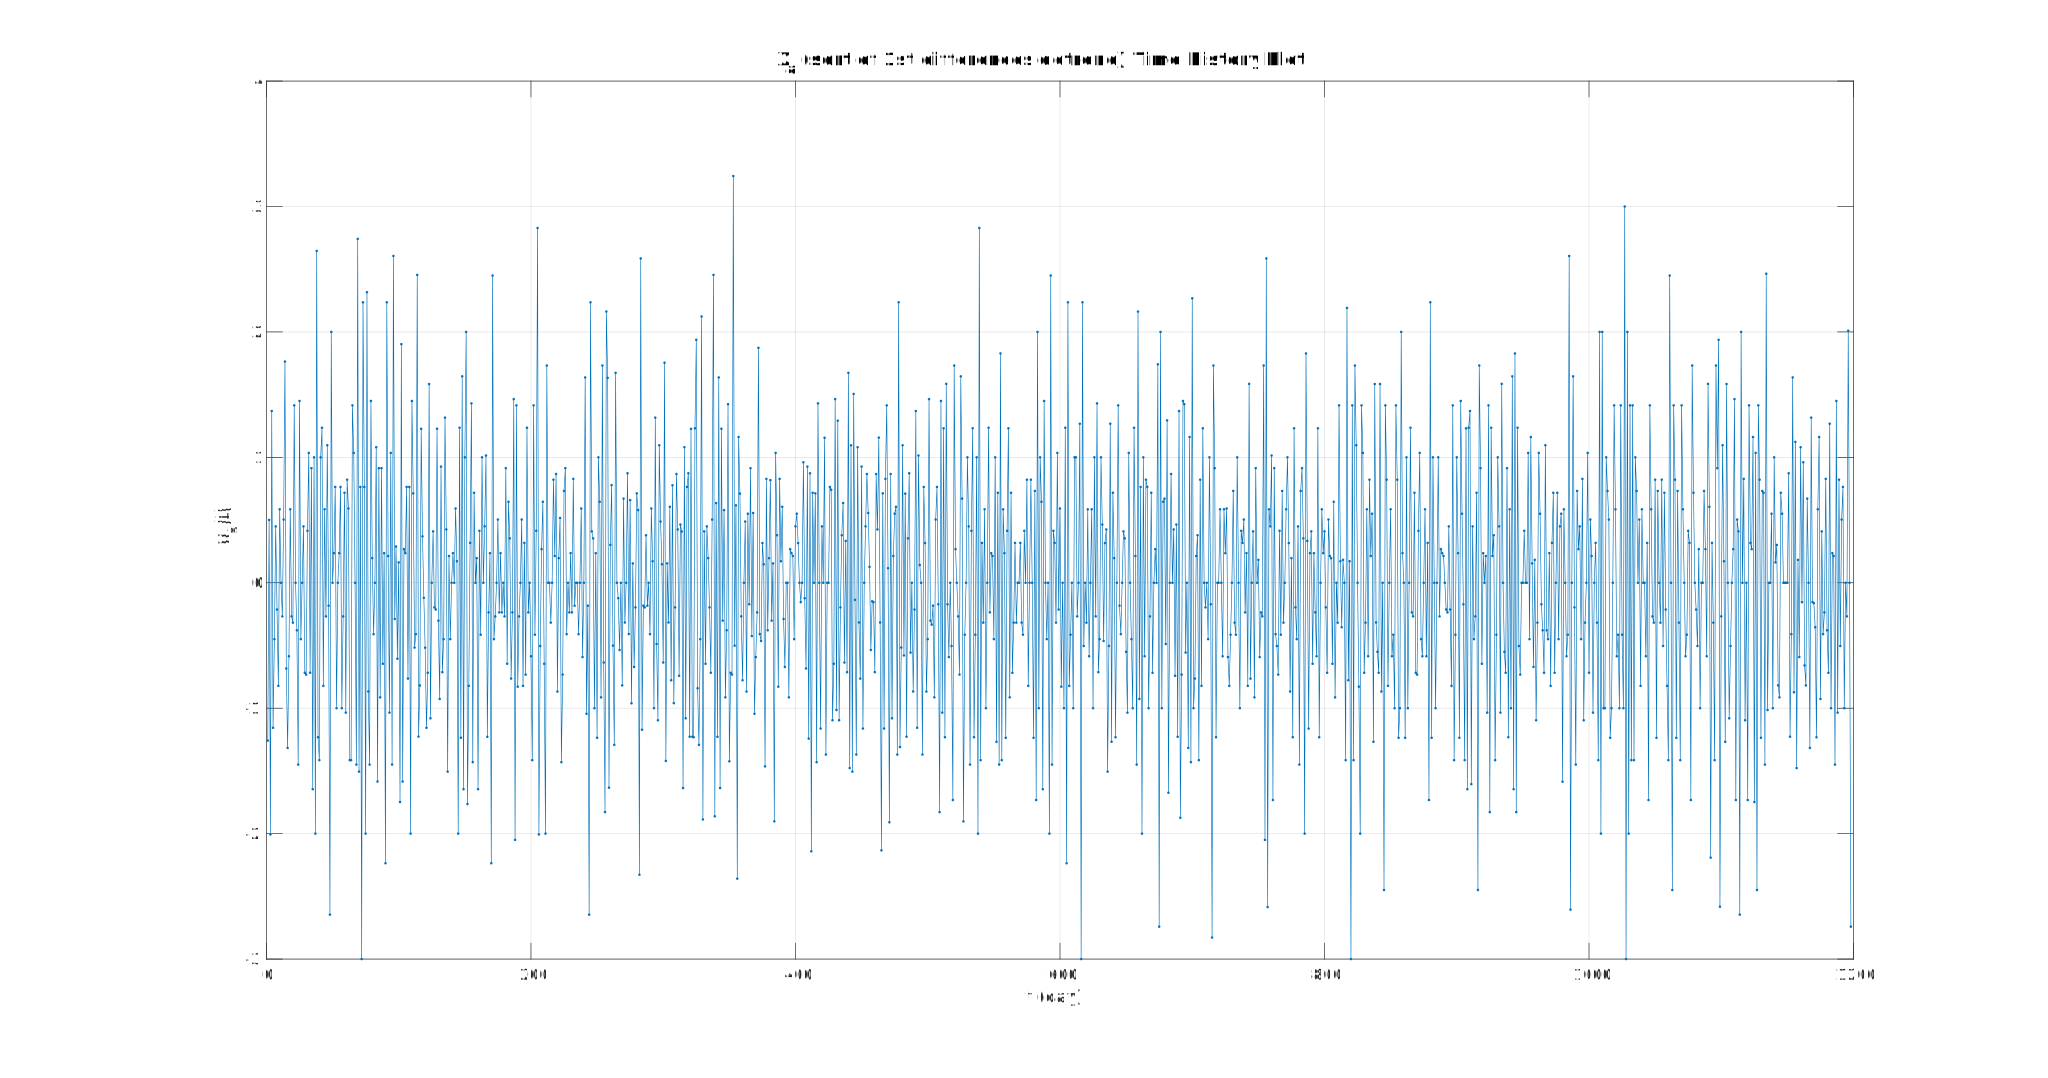
\includegraphics[width=\textwidth]{plots/xa_sqrt_of_1st_differences_history.svg.pdf}
        \caption{Διάγραμμα ιστορίας στη χρονοσειρά των πρώτων διαφορών των τετρ. ριζών, \emph{${X_a(t)}$}}
        \label{fig:xa_sqrt_of_1st_differences_history}
    \end{center}
\end{figure}

Για τη χροοσειρά των πρώτων διαφορών των τετραγωνικών ριζών που καταλήξαμε, παραθέτονται επίσης και τα διαγράμματα δειγματικής αυτοσυσχέτισης και δειγματικής μερικής αυτοσυσχέτισης με τα όρια σημαντικότητας (για εμπιστοσύνη 95\%):

\begin{figure}[H]
    \begin{center}
        \includegraphics[width=\textwidth]{assets/images/plots/xa_sqrt_of_1st_differences_autocorrelation.svg.pdf}
        \caption{Διάγραμμα (δειγματικής) αυτοσυσχέτισης της χρονοσειράς πρώτων διαφορών των τετραγωνικών ριζών, $r_x(\tau)$}
        \label{fig:xa_sqrt_of_1st_differences_autocorrelation}
    \end{center}
\end{figure}

\begin{figure}[H]
    \begin{center}
        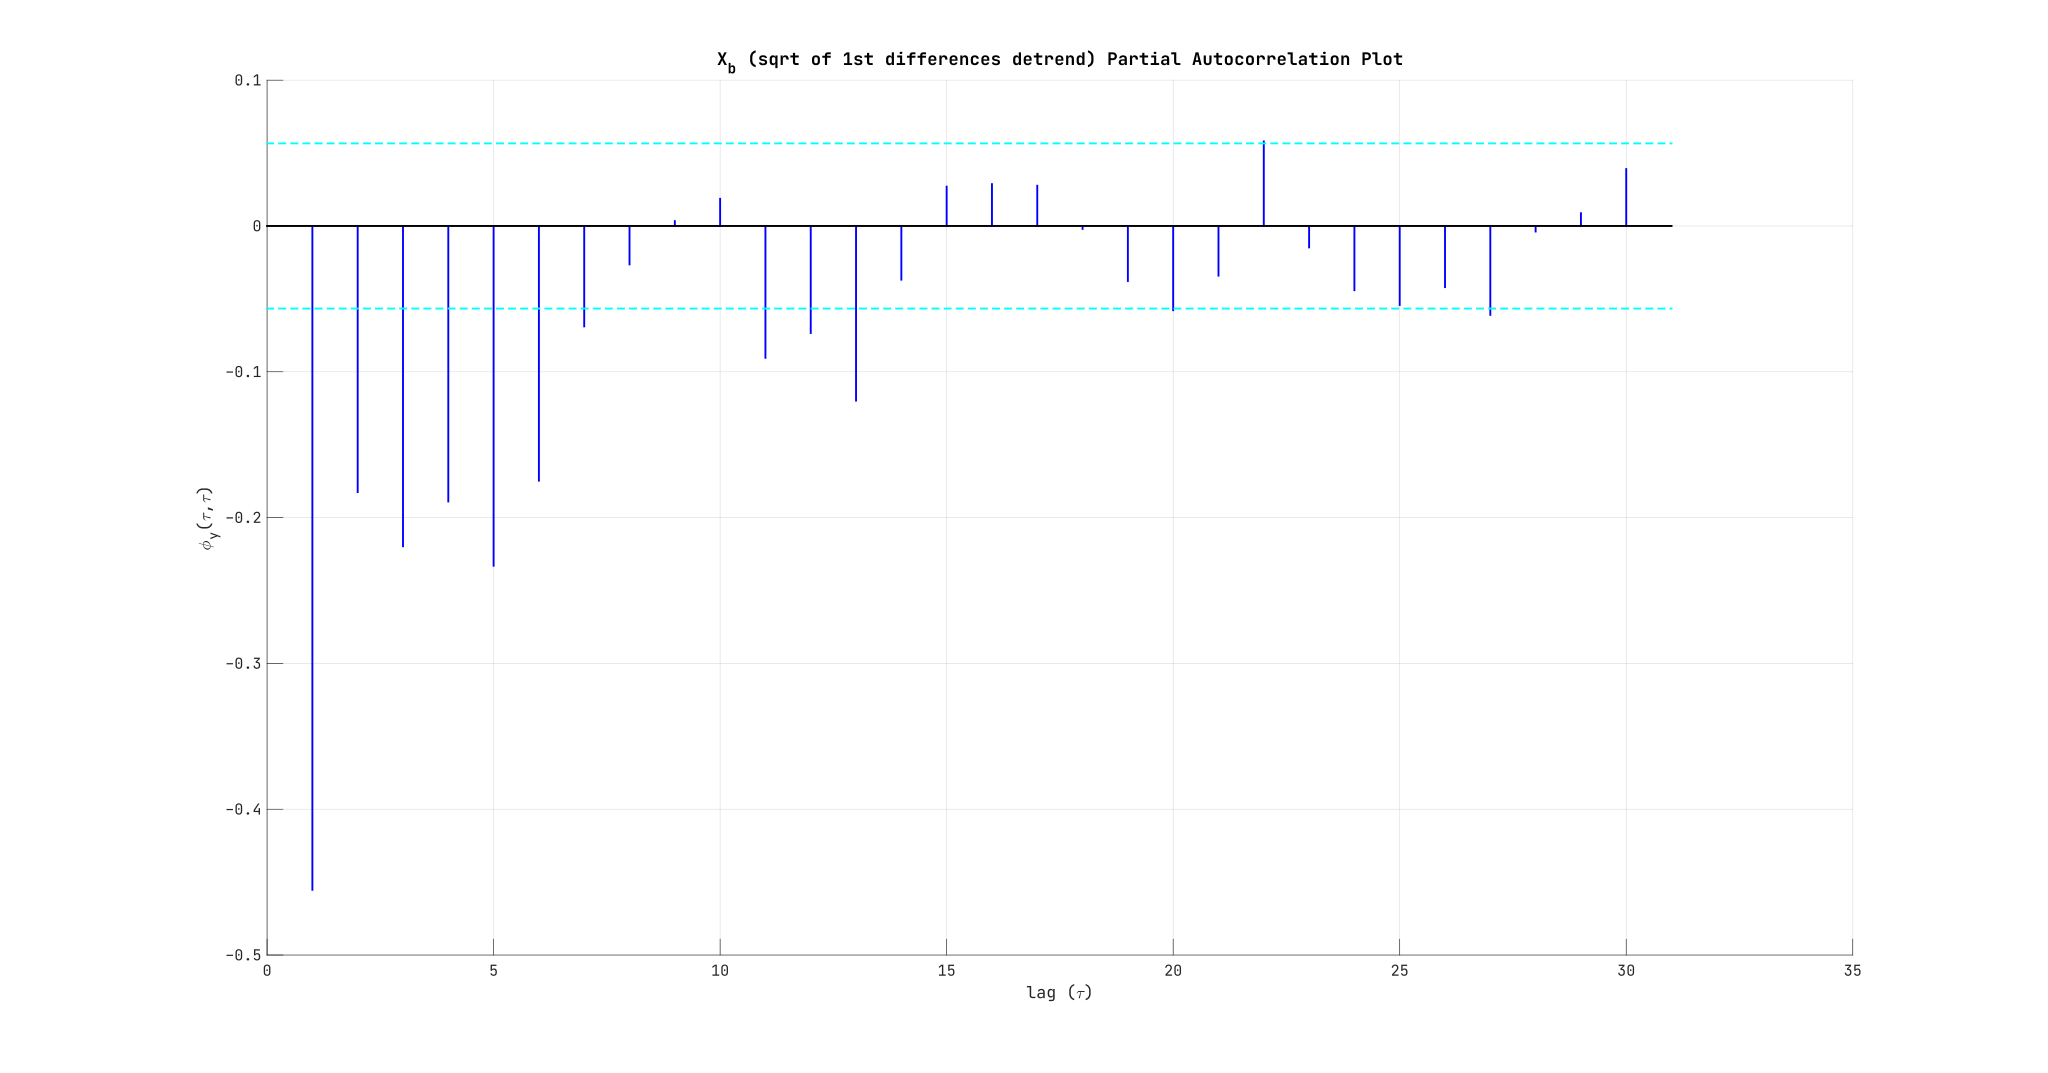
\includegraphics[width=\textwidth]{assets/images/plots/xb_sqrt_of_1st_differences_partial_autocorrelation.svg.pdf}
        \caption{Διάγραμμα (δειγματικής) μερικής αυτοσυσχέτισης της χρονοσειράς πρώτων διαφορών των τετραγωνικών ριζών, $\phi_x(\tau)$}
        \label{fig:xb_sqrt_of_1st_differences_partial_autocorrelation}
    \end{center}
\end{figure}

τα οποία όπως είναι αναμενόμενο είναι σχεδόν ίδια με τα αντίστοιχα της χρονοσειράς μόνο των πρώτων διαφορών της αρχικής (χωρίς δηλαδή το μετασχηματισμό της τετραγωνικής ρίζας), που δόθηκαν στα σχήματα \ref{fig:xa_1st_differences_autocorrelation} και \ref{fig:xa_1st_differences_partial_autocorrelation} παραπάνω.

